\section{Additional Information}
\label{sec:04_additionalInformation}

On top of the direction detection by \ac{TDOA}, additional information can be
extracted from the microphone data.
This information can be used to improve the single robot result or
to feed the team filter with information about the certainty of the \ac{WSDE} result.
As \cref{subsec:03_distance} has described, the distance of the sound source
can be estimated approximately for nearby signals that are aligned with
the x-axis of the robot's head.
Another intuitive approach is the inspection of the \ac{SNR} which
is expected to be higher for closer sound sources.
In addition, the \ac{PSNR} of the \ac{GCC} as defined in \cref{subsec:04_psnr} is
examined in detail.

\subsection{Distance Approximation}
\label{subsec:04_distance}

\Cref{subsec:03_distance} stated that the distance to a sound source
can be determined approximately if it comes from straight in front or
backwards of the robot.
Additionally, this calculation is only possible for sound sources that are
less than 0.66\si{\meter} in front or 15.3\si{\meter} behind in theory.
For this  case, a height of the sound source is estimated to be 1.5\si{\meter}.
To examine the validity of these assumptions, measurements from the front and
back of the robot are collected and evaluated among this range.
\Cref{tab:04_distance} lists the true distance as well as the distance estimate
for each measurement.
For both measurements with zero distance, the orientation of the whistle differs.
180\si{\degree} indicates that the whistle was turned in the opposite direction
of the robot.
In the other case (0\si{\degree}), the whistle was oriented unidirectional with the robot.
The distance is represented in robot coordinates, so that positive distance
expresses that the source was placed in front of the robot and oriented towards it
and vise versa.
\change[]{It might be more helpful to report errors here instead of the
	estimates, but it's not a big problem if you leave it like this.}
% -------------------------------------------------------------
\btline{ht}{1.2}
\btab{|c|c|c|c|c|c|}
\hline
No. & True Distance [\si{\meter}] & GCC Result [\si{\meter}] & CC Result [\si{\meter}] & Phase Result [\si{\meter}]\\
\hline
1 & +0.9 & $\infty$  & $\infty$ & $\infty$ \\
\hline
2 & +0.6 & $\infty$ & $\infty$ & $\infty$ \\
\hline
3 & +0.3 & 0.35 & 0.25 &  0.13 \\
\hline
4 & +0.0 (180\si{\degree}) & -0.13 & -0.15 & -0.23 \\
\hline
5 & -0.0 (0\si{\degree}) & 0.22 & 0.21 & 0.02 \\
\hline
6 & -0.3 & -0.15 & -0.27 & -0.45 \\
\hline
7 & -0.6 & -0.34 & -0.50 & -0.62 \\
\hline
8 & -0.9 & -0.70 & -0.91 & -0.99 \\
\hline
9 & -1.2 & -1.00 & -1.28 & -1.71 \\
\hline
10 & -1.5 & -1.39 & -1.59 & -2.98 \\
\hline
11 & -1.8 & -1.72 & -2.07 & -3.33 \\
\hline
12 & -2.1 & -2.16 & $\infty$ & -3.02\\
\hline
13 & -2.4 & -2.31 & $\infty$ & $\infty$ \\
\hline
14 & -3.75 & -3.66 & -9.51 & -4.15 \\
\hline
15 & -6.4 & -7.35 & -7.27 & $\infty$  \\
\hline
16 & -9.8 & $\infty$ & $\infty$ & $\infty$ \\
\hline
\etab
\et{Result of front and rear distance for all methods.}{04_distance}
% -------------------------------------------------------------

As the results show, that in many cases the distance can be approximated with
sufficiently small error.
One can see that the \ac{GCC} results are erroneous for small
distances, but gives a correct approximations that are not completely out of proportion
for all measurements except of the edge cases (no. 1, 2 and 16).
Compared to this, the \ac{CC} method performs better for small distances,
but fails completely for some measurements.
These failures of the \ac{CC} could be attributed to cases where the
lateral delays exceeded the maximum lateral samples to trigger the
distance estimation algorithm.
The phase difference method provides most incorrect results.
Especially measurement 10 stands out by being double the real value.

% \todo[inline]{Maybe you can show only the error statistics here and put the
% real measurements in the appendix?}

From the results one can say, that it is possible to estimate the distance
of a sound source by all methods but is mostly reliable for the \ac{GCC-PHAT} method.
Furthermore, the algorithm correctly detects sources that are out of
constructionally observable range.
However, for real cases one can not rely on the height parameter of the sound
source which varies according to the referee's body height.
Having this as approximation only, the distance result should be handled
with care.
Also if a localization algorithm is implemented for sound sources
at the same height as the robots' head, the distance estimation becomes unusable.

\subsection{SNR}
\label{subsec:04_snr}

Receiving information about the source location by the strength of a signal
is an intuitive approach.
Ideally, channels and robots that are closer to the sound source
receive greater signal data.
\Cref{subsec:03_snr} covers the implementation details about the \ac{SNR} which
is a value to expresses the strength of the signal compared to its background noise.
For the purpose of clarification, it is examined if channels
with larger \ac{SNR} are closer to the others on one single robot.
Additionally, this examination helps to ensure that the individual channels
are not biased towards internal noise of the robot's head.

Therefore, 3\si{\kilo\hertz} sinusoid signals are played back digitally from
0.73\si{\meter} distance and constant volume.
14 Measurements from different angles were taken with one robot.
Further evaluation is done by determining the channel with the maximum
\ac{SNR} between the channels.
It is expected that the nearest channel to the sound source has maximum \ac{SNR}.
At 85.71\si{\percent} of the measurements this assertion could be
evidenced.
In general, the \ac{SNR} seems to correlate in some extend with the
distance to the sound source and no channel seems to behave different
by nature.
To prove this relation for real whistle measurements, the same evaluation is
done with the laboratory-measurements.
By that, only 54.55\si{\percent} of the maximum \acp{SNR} match with the expected
channels.
This outcome is not sufficient to make conclusions about the signal source
direction on one robot.

From the multi-agent perspective, it would be a simple way to predict the sound
source position roughly if a relation between received signal strength on one robot
and distance to the source exists.
For example if multiple potential source positions exist for the multi-agent decision,
the \ac{SNR} information can used as subordinate indicator for the direction.
Another point is that information about the uncertainty of a \ac{WSDE} result
can be respected in the Bayesian updating algorithm straightforwardly.
Depending on the uncertainty, the covariance matrix of the incoming result can
be adjusted so that predictions that are assumed to have higher error have
a smaller influence to the posterior estimate.
In other words, \acp{SNR} of robots closer to the source would be higher
and to that effect, the reliability of their results is higher.
Thus, a relation between \ac{SNR} and distance on multi-agent level is examined in addition.

\unsure[]{IMHO a good practice is to report the number of experiments
	and/or have the data in the appendix (if you still have the data). But having
	it in the appendix is not super relevant. Don't waste time on it.}
% Thus, one intuitive hypothesis is assuming the existence of a relation between the
% received signal strength and distance to the source.

Taking the laboratory-measurements of \cref{subsec:04_labMeasurements}, this
hypothesis is examined by looking at the relation between distance and and the robots'
\ac{SNR} mean over all channel which is now called \textit{robot-\ac{SNR}}.
Because the whistle is not blown equally for all laboratory-measurements,
the robot-\ac{SNR} is scaled by the overall mean of all robots' \acp{SNR} for each
measurement (named \textit{measurement-\ac{SNR}}).
% $\text{Relative SNR} = \frac{SNR_{robot}}{Mean(SNR_{measurement})}$.
\Cref{fig:04_snrDistance} presents the relations between distance of a robot
and the robots-\ac{SNR} relative to the measurement-\ac{SNR}.

Looking at the plot, no straightforward link between both values can be found.
Calculating the correlation coefficient $\rho$ between both quantities,
its value is -0.2860.
This outcome verifies that no simple connection between \ac{SNR} and distance
can be placed.

For the real whistle measurements, no assuring relation between \ac{SNR}
and distance to source can be found neither between the microphone
channels on the robots' head nor between the single robots.
Consequentially, one must assume that the environmental circumstances
like multi-path propagation and reflection have large influence
on the signal data.
Thus, the \ac{SNR} will not utilized as additional information
for the \ac{WSDE} algorithm nor for the multi-agent filter.
% -------------------------------------------------------------
\begin{figure}[h]
	\centering
	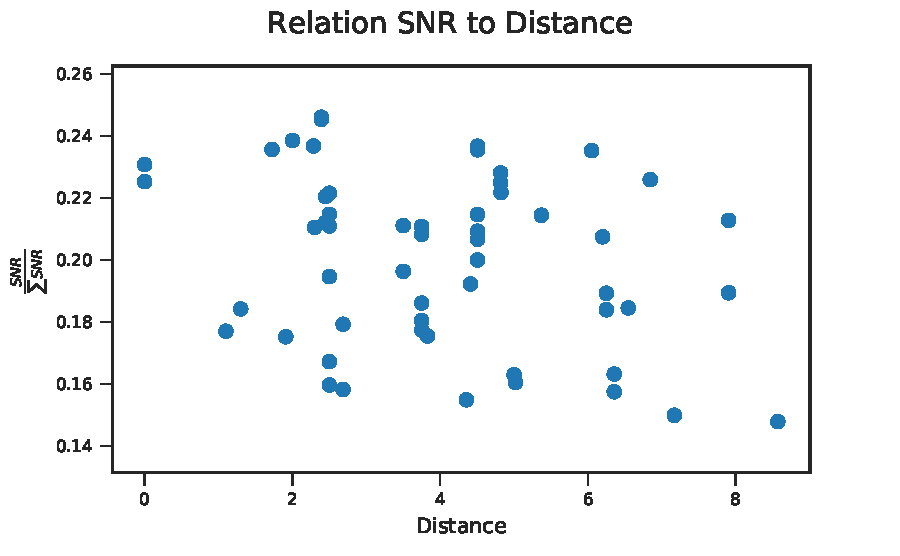
\includegraphics[]{figures/evaluation/snr_scatter}
	\caption{Visualization of relation between SNR and distance.}
	\label{fig:04_snrDistance}
\end{figure}
% -------------------------------------------------------------

\subsection{PSNR}
\label{subsec:04_psnr}

As referred in \cref{sec:02_gcc}, the main characteristic of the \ac{GCC-PHAT}
algorithm is the emerging sharp peak compared to \ac{CC} functions.
\Cref{fig:02_gccTheory} illustrates this characteristic for the ideal case where
two similar, but shifted signals with normally distributed noise are
input signals of the \ac{GCC} algorithm.
However, with real whistle data the \ac{GCC} function does not always
output a strong peak.
This is a known topic and there exists research that inspects how to handle
the ambiguity of \ac{GCC} functions like \cite{optimal_peak_localization} does.
Exemplary \cref{fig:04_psnrExample} shows such a case where the \ac{GCC} does not produce
a clear result.
% -------------------------------------------------------------
\begin{figure}[h]
	\centering
	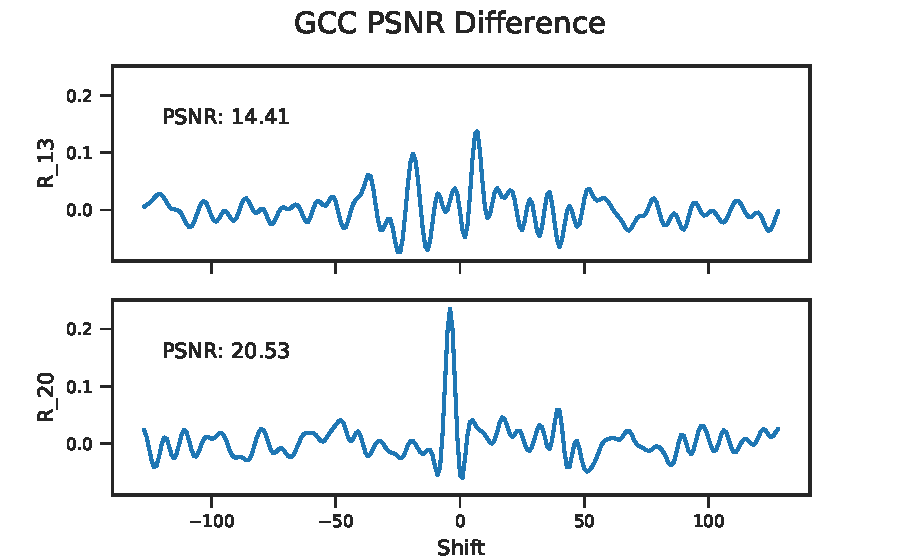
\includegraphics[]{figures/evaluation/psnr_example}
	\caption{}
	\label{fig:04_psnrExample}
\end{figure}
% -------------------------------------------------------------

$R_{13}$ and $R_{20}$ represents \ac{GCC} functions of the same measurement
but between different channels.
As the plot shows, the \ac{GCC} between channels 2 and 0 yields an outcome
with a easily recognizable peak.
In comparison, the peak of the upper plot which is the \ac{GCC} between channels 1 and 3
is less distinguishable from the remaining part.


In conclusion, one can assume that the lack of a sharp peak indicates
a less valid delay result of the \ac{GCC}.
The next sections covers the validity of this hypothesis by first evaluating
if the \ac{PSNR} can help with the selection of the frames used in the \ac{WSDE}.
On the other hand the informative value contained in the \ac{PSNR} regarding the
overall \ac{WSDE} on one robot is examined.

\subsubsection*{Frame Selection}

One perspective is to insert the PSNR information into the \ac{WSDE} of
individual robots.
In \cref{fig:04_psnr2FrameShift}, the frame to examine is
shifted before and after a manually defined signal start index.
The robot was positioned at the center point
while the whistle is blown at -33.7\si{\degree} with 4.5\si{\meter}
distance.
The frame size of the \ac{GCC} is set to the default size of 256 samples and
the window shift samples are quarter of the frame size.
% -------------------------------------------------------------
\begin{figure}[h]
	\centering
	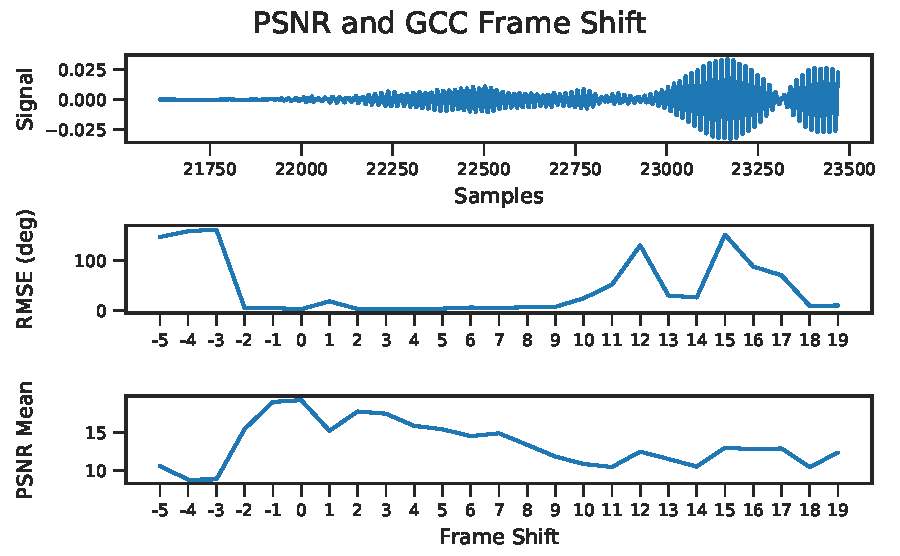
\includegraphics[]{figures/evaluation/gcc_frame_shift}
	\caption{
		Relation between \ac{PSNR}
		and selection of the frame in time. Signal data
		of the rear left channel is plotted in the upper window.
		In this measurement, the whistle is positioned at right front
		of the robot.
	}
	\label{fig:04_psnr2FrameShift}
\end{figure}
% -------------------------------------------------------------
For better understanding, samples of the front right channel are plotted
in the upper graph of \cref{fig:04_psnr2FrameShift}.
The second graph shows the \ac{RMSE} of the robot direction result
over the frame shifts.
For the lower graph, the mean over the \acp{PSNR} of all channels
is presented.
As a general trend, it can be observed that the error of the predicted
direction is low for frame shifts with a high \ac{PSNR}.
This confirms the hypothesis stated early in this section.
For shifts smaller than -2, the whistle signal does not intersect with the
evaluated frames.
Therefore, the prediction error in this regime is high.
An important notice is that the \ac{PSNR} decays as the frame is shifted towards
later samples on the whistle signal. This indicates that the implemented
\ac{GCC-PHAT} method is not suitable for arbitrary subsamples of the signal.
% Without additional information about the rough direction,
% ambiguity exists due to periodicity of the signal.
% Due to the inconclusive result of the \ac{SNR} in \cref{subsec:04_snr}
% one decides not to take the signal magnitude as such information
% into account.
% Thus, the decisive role of the start of the signal is underlined again.
% -------------------------------------------------------------

\subsubsection*{Informative Value}

In this section, the \ac{PSNR} value of one \ac{GCC-PHAT} calculation is brought
into comparison with the error of the direction angle resulting from the delay.
% Two cases of errors are taken into consideration.
In the following, the \ac{PSNR} is referred to as high if it exceeds 17.5
whereat the \ac{PSNR} value ranges from 10.1 to 28.8 for measurements in
\cref{subsec:04_labMeasurements}.

First, for each channel pair the error between true direction of the signal source
and the direction candidate with smaller angle error emerging from the \ac{GCC}
delay are put into context.
The results are grouped into two classes based on the associated \ac{PSNR} value.
If the \ac{PSNR} of the \ac{GCC} is greater than the threshold of 17.5,
the angular error of its source direction result is classified as high \ac{PSNR}.
Else, it pertains to the errors with low \ac{PSNR}.
Out of a total number of 220 measurements, 78 correlations reported a
\ac{PSNR} below the threshold. The \ac{RMSE} of all source directions within this
group was 35.77\si{\degree}.
Compared to this, the \ac{RMSE} of the remaining 144 measurements
is 15.86\si{\degree} only.

To see the impact on a complete robot result, the same evaluation is done
with the final angular errors of the robots' \acp{WSDE}.
Here, the \ac{PSNR} value is the mean over all channel pairs' \acs{PSNR}.
The angular \ac{RMSE} of the direction classified as low \ac{PSNR} value
are larger with 21.15\si{\degree} whereat the error of the high \ac{PSNR} case
is 9.1\si{\degree}.

From the results one can find a relation between \ac{PSNR} and validity of a
computed delay between two channels with the \ac{GCC-PHAT} method.
Within this work the  \ac{PSNR} information is not included for the implementation
of the multi-agent decision, but for the \ac{WSDE} of a single robot.
Thus, the frames for the \ac{GCC} algorithm to compute the delay between the channels
are selected by the highest \ac{PSNR} mean value in a range around the start index.
The implementation is explained in \cref{subsec:03_directionEstimation} in further detail.
